
\documentclass[12pt,a4paper]{article}
\usepackage[utf8]{inputenc}
\usepackage[T1]{fontenc}
\usepackage[brazil]{babel}
\usepackage{amsmath,amssymb,amsfonts}
\usepackage{graphicx}
\usepackage{booktabs}
\usepackage{hyperref}
\usepackage{minted}
\usepackage{tocloft}
\usepackage{geometry}
\usepackage{csvsimple}
\geometry{margin=2.5cm}
\usepackage{siunitx}
\sisetup{
  round-mode=places,
  round-precision=9,
  table-number-alignment=center,
  detect-all,
  scientific-notation=true
}

\title{PCS5029/PTC5725 -- Aula 06\\\large Introdução aos Métodos Espectrais}
\author{Renan de Luca Avila}
\date{\today}

\begin{document}
\begin{titlepage}
\centering

\includegraphics[width=0.35\textwidth]{EP.jpg}\par\vspace{1cm}
{\scshape\LARGE Escola Politécnica da Universidade de São Paulo\par}
\vspace{1.5cm}
{\huge\bfseries Aula 07 -- Métodos Espectrais\par}
\vspace{0.5cm}
{\Large Resolução da tarefa\par}
\vfill
{\large Renan de Luca Avila\par}
{\large \today\par}
\end{titlepage}

\tableofcontents
\newpage

\section{Resumo}
Este relatório implementa, em Python, os exercícios apresentados nos slides da Aula 07 (Prof.\ Osvaldo Guimarães), e discute as soluções. O documento contém códigos completos, figuras e tabelas, além de apêndices com setup e fontes.

% \subsection{Exercício X}

% \subsubsection{Enunciado}
% % Descreva o enunciado aqui com os detalhes matemáticos

% \subsubsection{Planejamento e fundamentos teóricos}
% % Descreva o plano para resolver o problema e cite os fundamentos teóricos que sustentam o plano, incluindo fórmulas e equações justificando o caminho escolhido

% \subsubsection{Etapas de implementação e funções principais}
% % Coloque citações de trechos do código aqui e explique o que cada uma delas faz relacionando com os fundamentos teóricos (use minted copiando trechos de código diretamente). Coloque trechos e os explique um a um, não coloque o código completo, pois este estará no apêndice referenciando o arquivo na pasta /code.

% \subsubsection{Resultados e discussão}
% % Coloque aqui figuras (da pasta /figures) e tabelas (da pasta /tables) que mostrem os resultados obtidos como saída do código e interprete os resultados

% \subsubsection{Conclusão}
% % Resuma o que fizemos para resolver e conclua com avaliações dos resultado

\section{Exercício 1 — Integrais numéricas por quadraturas espectrais de Legendre e Chebyshev}

\subsection{Enunciado}
Nesta tarefa, foi solicitado o cálculo numérico de quatro integrais reais em intervalos finitos, utilizando métodos espectrais de quadratura de alta precisão.  
O objetivo é comparar a eficiência e a taxa de convergência das regras de Gauss–Legendre, Gauss–Lobatto, Gauss–Radau e duas variantes baseadas em polinômios de Chebyshev (Fejér I e Clenshaw–Curtis).

As integrais propostas são:
\[
\begin{aligned}
I_1 &= \int_{0}^{4} t\,e^{2t}\,dt,\\[4pt]
I_2 &= \int_{-1}^{0} \frac{\sin x}{x}\,dx,\\[4pt]
I_3 &= \int_{0}^{2} e^{x^{2}}\,dx,\\[4pt]
I_4 &= \int_{0}^{1} \frac{e^{x-1}-1}{x-1}\,dx.
\end{aligned}
\]

A precisão desejada é de erro relativo inferior a $10^{-8}$, sendo cada integral avaliada com $n = 4,\,8,\,16,\,32$ pontos para cada método.  
Os resultados numéricos devem ser comparados com valores de referência analíticos (quando disponíveis) ou obtidos por integração de alta precisão via \texttt{mpmath.quad}.

\subsection{Planejamento e fundamentos teóricos}
A integração numérica de uma função $f(x)$ em um intervalo $[a,b]$ é aproximada por:
\[
\int_a^b f(x)\,dx \approx \sum_{i=1}^{n} w_i\,f(x_i),
\]
onde $\{x_i\}$ são os \emph{nós} e $\{w_i\}$ os \emph{pesos} da quadratura.

\paragraph{Fundamentos (Legendre).}
As regras de Gauss–Legendre, –Lobatto e –Radau usam propriedades de ortogonalidade de $P_n(x)$:
\[
\int_{-1}^{1} P_m(x)P_n(x)\,dx = \frac{2}{2n+1}\,\delta_{mn}.
\]
Fórmulas clássicas:
\[
\text{Gauss: } w_i = \frac{2}{(1-x_i^2)\,[P_n'(x_i)]^2},\qquad
\text{Lobatto: } w_i = \frac{2}{n(n-1)\,[P_{n-1}(x_i)]^2},
\]
\[
\text{Radau (nó em $-1$): } w_i = \frac{1-x_i}{n^2\,[P_{n-1}(x_i)]^2}.
\]
Para aplicar em $[a,b]$, mapeamos $z\in[-1,1] \mapsto x=\tfrac{b-a}{2}z+\tfrac{b+a}{2}$ e $w=\tfrac{b-a}{2}w_z$.

\paragraph{Fundamentos (Chebyshev).}
Fejér I e Clenshaw–Curtis usam $T_k(x)=\cos(k\arccos x)$ com nós
\[
x_k=\cos\!\Big(\frac{(2k-1)\pi}{2n}\Big) \quad\text{(Fejér I)},\qquad
x_k=\cos\!\Big(\frac{k\pi}{n}\Big) \quad\text{(Clenshaw–Curtis)},
\]
e pesos obtidos por somas de cossenos (séries de Fourier discretas).

\paragraph{Soluções analíticas de referência.}\mbox{}\\

\textbf{(a) } $I_1=\displaystyle\int_0^4 t e^{2t}\,dt$. Integração por partes com
$u=t,\; dv=e^{2t}\,dt\Rightarrow du=dt,\; v=\tfrac{1}{2}e^{2t}$:
\[
\int t e^{2t}\,dt = \frac{t}{2}e^{2t}-\int \frac{1}{2}e^{2t}\,dt
= \frac{t}{2}e^{2t}-\frac{1}{4}e^{2t}+C.
\]
Logo
\[
I_1 = \Big[\frac{t}{2}e^{2t}-\frac{1}{4}e^{2t}\Big]_{0}^{4}
= \frac{7}{4}e^{8}-\Big(-\frac{1}{4}\Big)=\frac{1}{4}\big(7e^{8}+1\big).
\]

\vspace{1cm}

\textbf{(b) } $I_2=\displaystyle\int_{-1}^{0}\frac{\sin x}{x}\,dx$. Note que $\frac{\sin x}{x}$ é par, então
\[
I_2=\int_{-1}^{0}\frac{\sin x}{x}\,dx=\int_{0}^{1}\frac{\sin x}{x}\,dx
=\operatorname{Si}(1),
\]
onde $\operatorname{Si}(x)=\int_0^x \frac{\sin t}{t}\,dt$ é a integral do seno.

\vspace{1cm}

\textbf{(c) } $I_3=\displaystyle\int_{0}^{2}e^{x^2}\,dx$. Não há primitiva elementar, mas
\[
\int e^{x^2}\,dx=\frac{\sqrt{\pi}}{2}\,\operatorname{erfi}(x),\qquad
\operatorname{erfi}(x)=\frac{2}{\sqrt{\pi}}\int_0^x e^{t^2}\,dt.
\]
Assim,
\[
I_3=\frac{\sqrt{\pi}}{2}\,\operatorname{erfi}(2).
\]

\vspace{1cm}

\textbf{(d) } $I_4=\displaystyle\int_{0}^{1}\frac{e^{x-1}-1}{x-1}\,dx$. Com $u=x-1$ (de $-1$ a $0$):
\[
I_4=\int_{-1}^{0}\frac{e^{u}-1}{u}\,du
=\sum_{k=1}^{\infty}\frac{1}{k!}\int_{-1}^{0}u^{k-1}\,du
=\sum_{k=1}^{\infty}\frac{1}{k!}\Big[\frac{u^{k}}{k}\Big]_{-1}^{0}
=\sum_{k=1}^{\infty}\frac{(-1)^{k+1}}{k\,k!}.
\]
Usando a expansão de $\operatorname{Ei}(x)$:
\[
\operatorname{Ei}(x)=\gamma+\ln|x|+\sum_{k=1}^{\infty}\frac{x^{k}}{k\,k!},
\]
obtemos, para $x=-1$,
\[
\sum_{k=1}^{\infty}\frac{(-1)^{k+1}}{k\,k!}=\gamma-\operatorname{Ei}(-1).
\]
Portanto,
\[
I_4=\gamma-\operatorname{Ei}(-1),
\]
onde $\gamma$ é a constante de Euler–Mascheroni.

\subsection{Etapas de implementação e funções principais}
A implementação em \texttt{Python 3.11} segue fielmente as fórmulas acima. Abaixo, destacamos trechos essenciais (o \textbf{código completo} está no apêndice do relatório, arquivo \texttt{/code/aula07\_tarefa1\_quadraturas.py}).

\paragraph{Mapeamento $[-1,1]\to[a,b]$ e integração genérica.}
\begin{minted}[fontsize=\footnotesize,breaklines]{python}
def map_to_interval(z, w, a, b):
    x = 0.5*((b-a)*z + (b+a))
    ww = 0.5*(b-a)*w
    return x, ww

def integrate_rule(f, a, b, rule, n):
    z, w = nodes_weights(rule, n)   # despacha p/ regra escolhida
    x, ww = map_to_interval(z, w, a, b)
    return float(np.sum(ww * f(x)))
\end{minted}
\emph{Comentário.} Implementa o mapeamento linear e a soma $\sum_i w_i f(x_i)$.

\paragraph{Gauss–Lobatto: $x=\{-1,\,\text{raiz de }P'_{n-1},\,1\}$; $w=\tfrac{2}{n(n-1)P_{n-1}(x)^2}$.}
\begin{minted}[fontsize=\footnotesize,breaklines]{python}
def gauss_lobatto(n):
    z = np.empty(n); z[0], z[-1] = -1.0, 1.0
    if n > 2:
        P = np.polynomial.legendre.Legendre([0]* (n-1) + [1.0])
        roots = np.sort(P.deriv().roots())
        z[1:-1] = roots
    Pn1 = np.polynomial.legendre.Legendre([0]* (n-1) + [1.0])(z)
    w = 2.0 / ((n-1)*n*(Pn1**2))
    return z, w
\end{minted}
\emph{Comentário.} Usa as raízes de $P'_{n-1}$ e aplica a fórmula de pesos clássica.

\paragraph{Gauss–Radau (nó fixo em $-1$) via matriz tridiagonal (Jacobi).}
\begin{minted}[fontsize=\footnotesize,breaklines]{python}
def gauss_radau_left_tridiag(n):
    j = np.arange(0, n-1)
    alpha = 1.0 / ((2*j+1)*(2*j+3))
    j2 = np.arange(1, n-1)
    beta = np.sqrt(j2*(j2+1.0)) / (2*j2+1.0)
    M = np.diag(alpha) + np.diag(beta,1) + np.diag(beta,-1)
    vals, _ = np.linalg.eigh(M)
    z = np.concatenate(([-1.0], vals))        # nós (inclui -1)
    Pn1 = np.polynomial.legendre.Legendre([0]* (n-1) + [1.0])(z)
    w = (1.0 - z) / (n**2 * (Pn1**2))         # pesos
    return z, w
\end{minted}
\emph{Comentário.} Replica a construção de Radau do material do professor (base Legendre $\Rightarrow$ tridiagonal simétrica).

\paragraph{Clenshaw–Curtis (Chebyshev–Lobatto) $x_k=\cos\!\frac{k\pi}{n}$; pesos por somas de cossenos.}
\begin{minted}[fontsize=\footnotesize,breaklines]{python}
def clenshaw_curtis(n):
    N = n - 1
    theta = np.pi * np.arange(0, N+1) / N
    z = -np.cos(theta)
    w = np.zeros(n)
    if N % 2 == 0:
        w[0] = w[-1] = 1.0/(N**2 - 1)
        v = np.ones(n-2)
        for k in range(1, N//2):
            v -= 2*np.cos(2*k*theta[1:-1])/(4*k*k - 1)
        v -= np.cos(N*theta[1:-1])/(N**2 - 1)
        w[1:-1] = 2*v/N
    else:
        w[0] = w[-1] = 1.0/N**2
        v = np.ones(n-2)
        for k in range(1, (N+1)//2):
            v -= 2*np.cos(2*k*theta[1:-1])/(4*k*k - 1)
        w[1:-1] = 2*v/N
    return z, w
\end{minted}
\emph{Comentário.} Implementa a fórmula $O(N^2)$ padrão (Trefethen) para CC.

\paragraph{Integrais de teste e referências (conectando às soluções analíticas).}
\begin{minted}[fontsize=\footnotesize,breaklines]{python}
def I1_ref():  # (1/4)(7 e^8 + 1)
    F = lambda t: 0.25*np.exp(2*t)*(2*t - 1)
    return float(F(4) - F(0))

def I2_ref():  # Si(1)
    return float(mp.si(1))

def I3_ref():  # (sqrt(pi)/2) erfi(2)
    return float(0.5*math.sqrt(math.pi)*mp.erfi(2))

def I4_ref():  # gamma - Ei(-1)
    return float(mp.euler - mp.ei(-1))
\end{minted}
\emph{Comentário.} Cada função referencia exatamente as expressões demonstradas na seção analítica.

\subsection{Resultados e discussão}
As Figuras~\ref{fig:conv_I1}–\ref{fig:conv_I4} exibem curvas de \emph{erro relativo} em escala log--log, e as Tabelas~\ref{tab:errors_I1}–\ref{tab:errors_I4} apresentam os valores numéricos por método e $n$.

\begin{figure}[h!]\centering
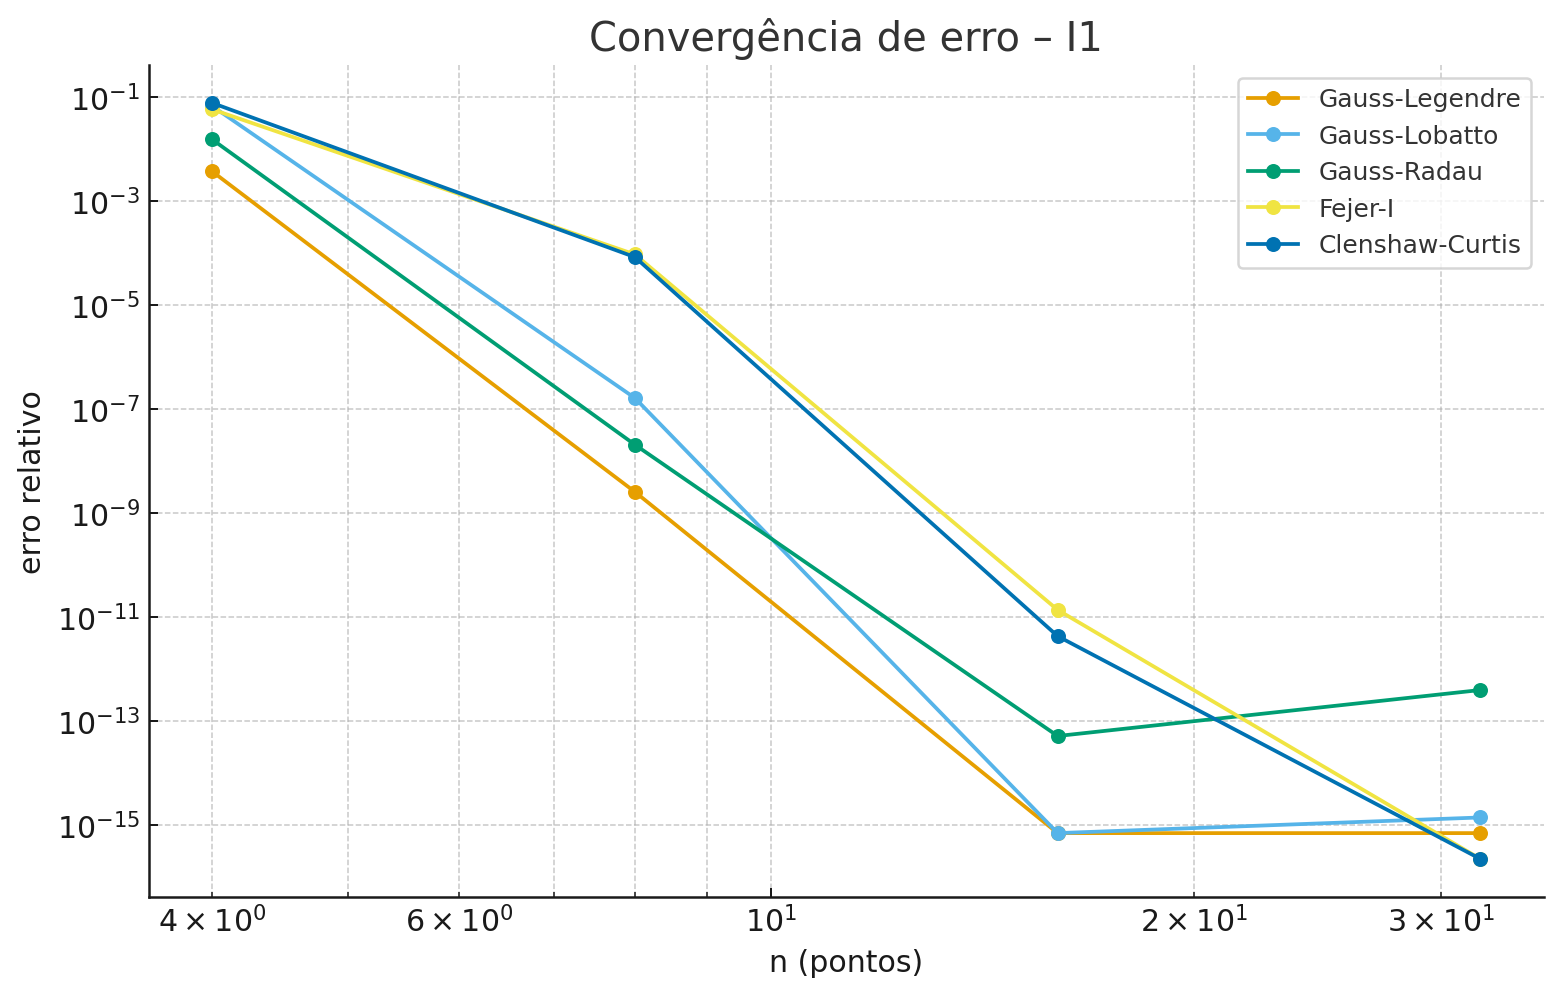
\includegraphics[width=\textwidth]{figures/convergence_I1.png}
\caption{Convergência de erro para $I_1 = \int_0^4 t e^{2t}\,dt$.}\label{fig:conv_I1}
\end{figure}

\begin{figure}[h!]\centering
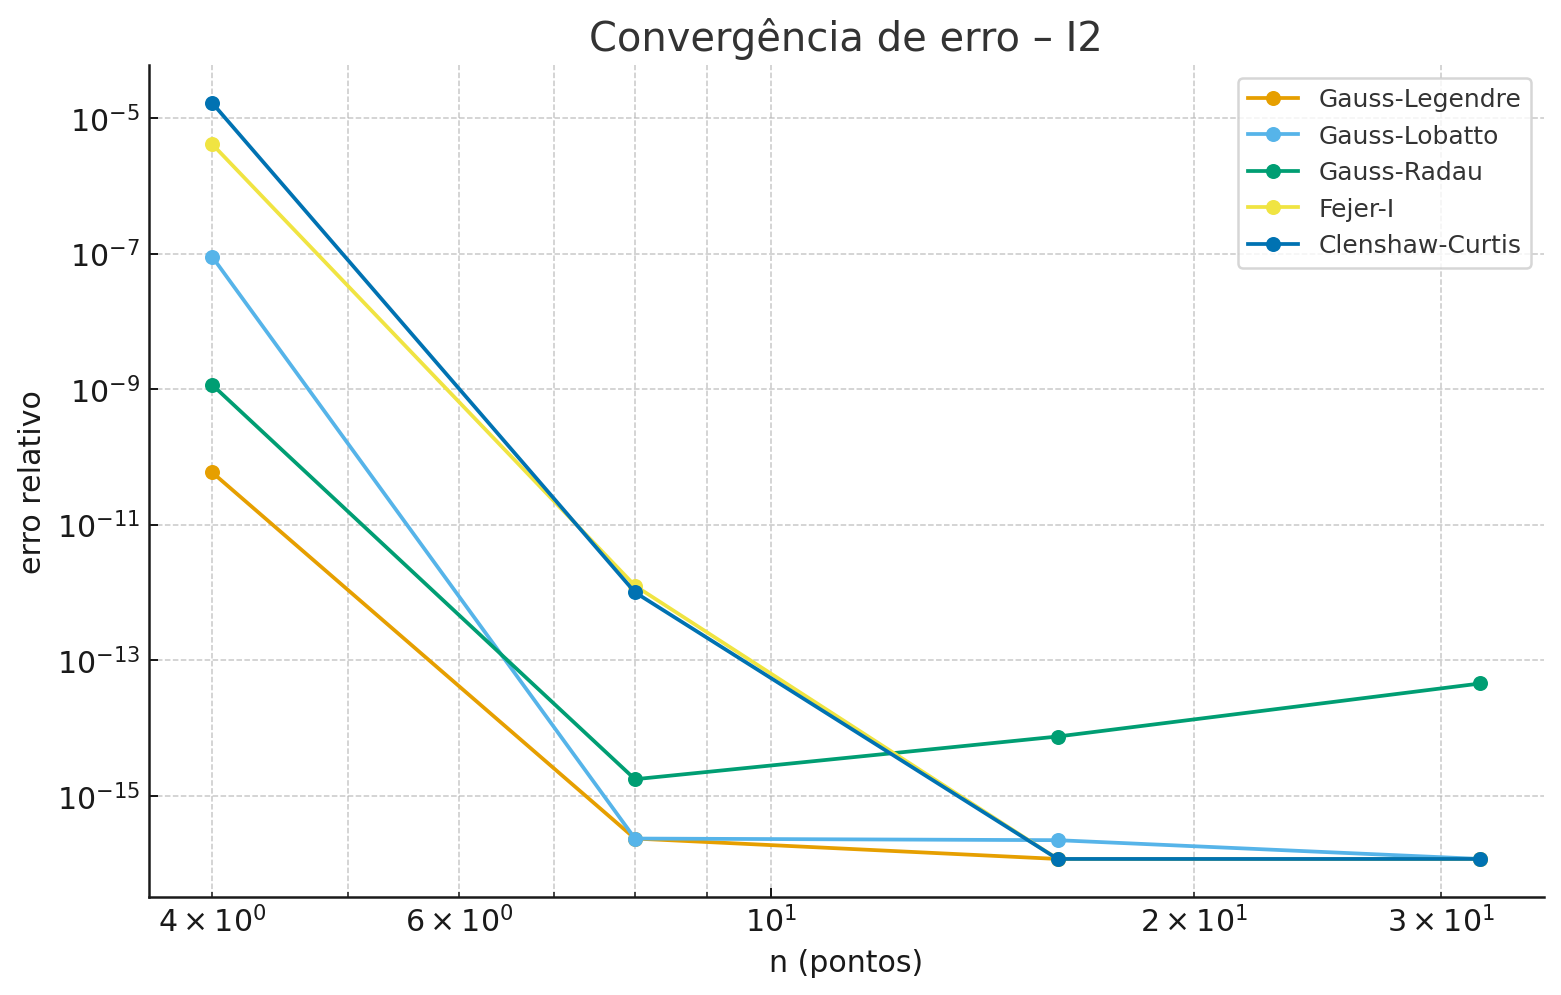
\includegraphics[width=\textwidth]{figures/convergence_I2.png}
\caption{Convergência de erro para $I_2 = \int_{-1}^0 \frac{\sin x}{x}\,dx$.}\label{fig:conv_I2}
\end{figure}

\begin{figure}[h!]\centering
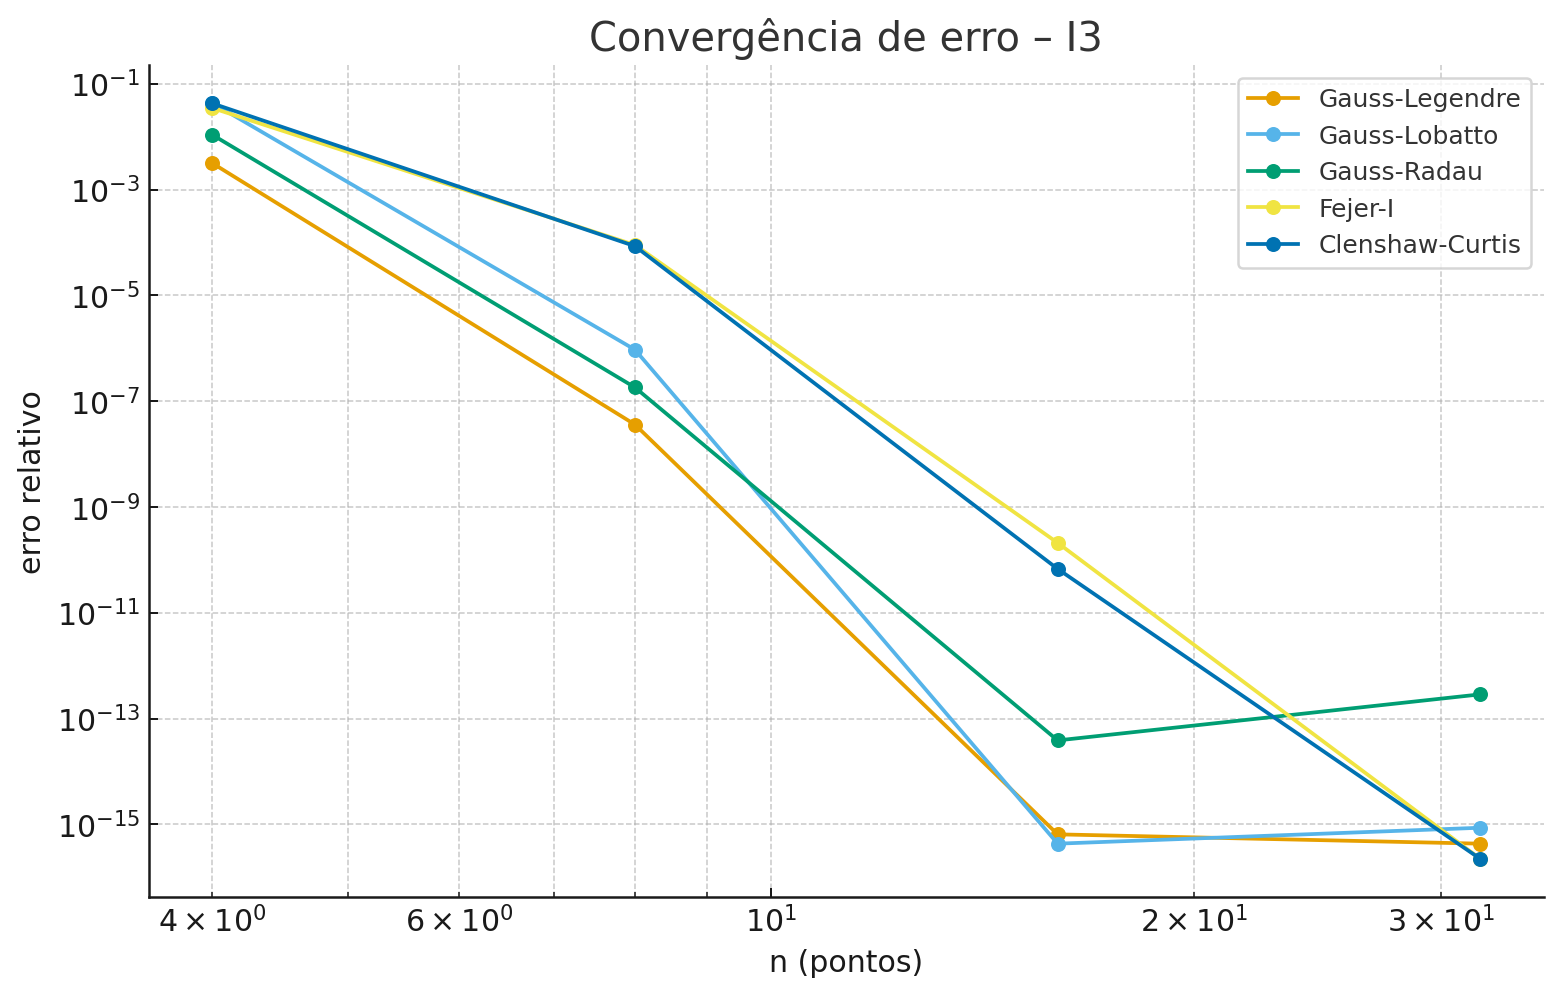
\includegraphics[width=\textwidth]{figures/convergence_I3.png}
\caption{Convergência de erro para $I_3 = \int_0^2 e^{x^2}\,dx$.}\label{fig:conv_I3}
\end{figure}

\begin{figure}[h!]\centering
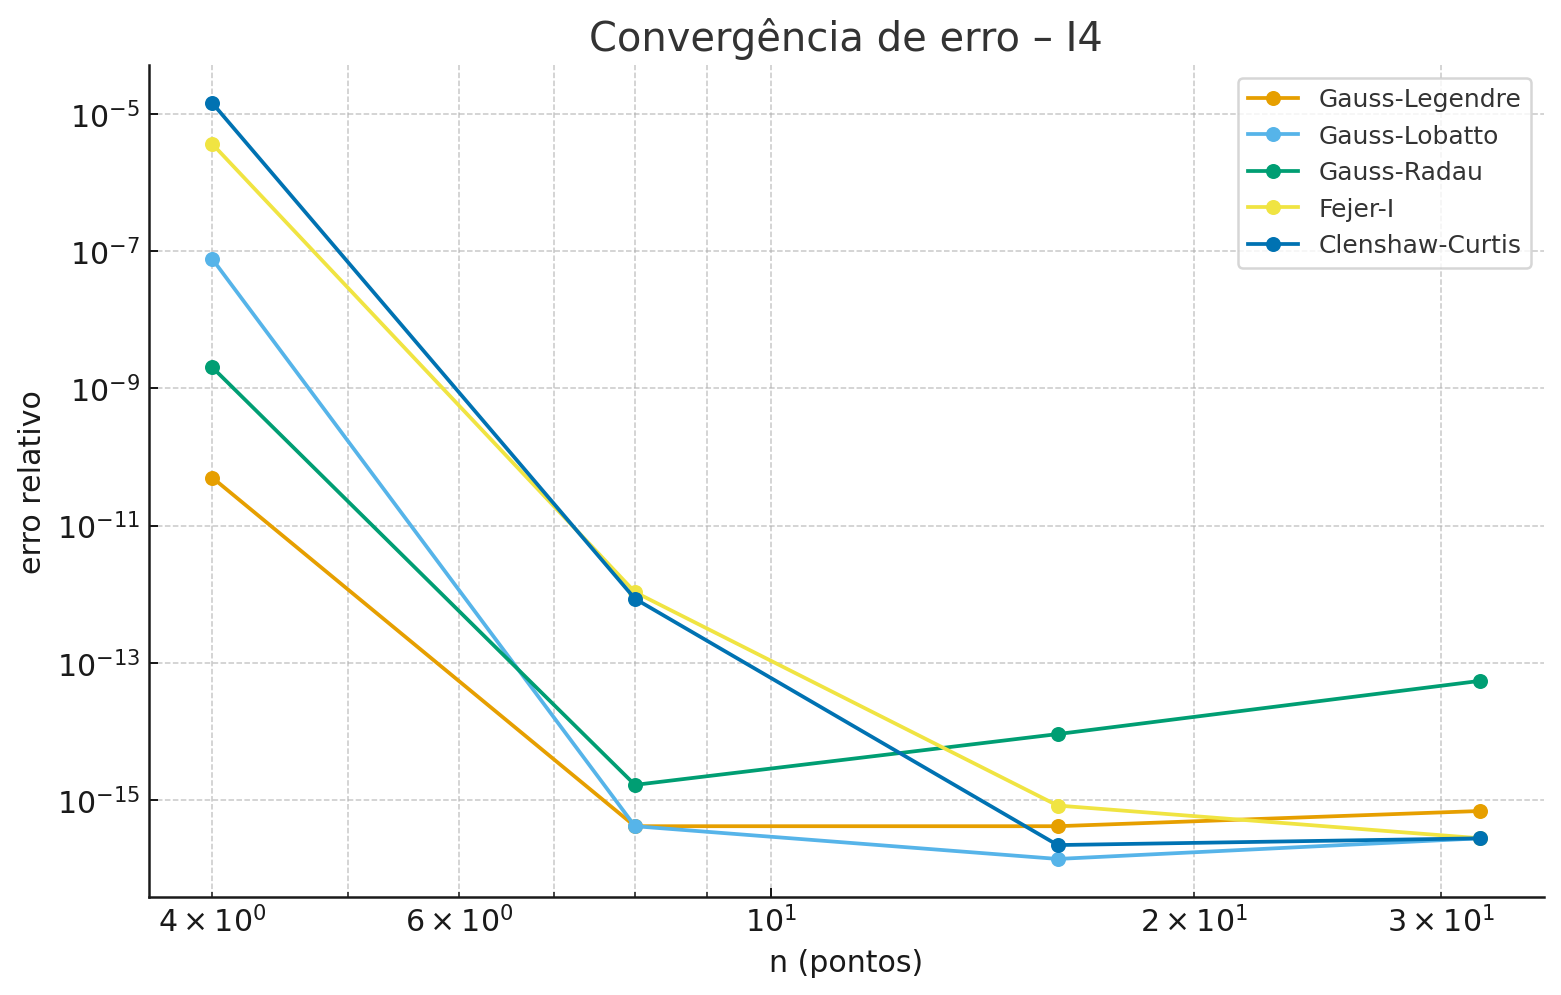
\includegraphics[width=\textwidth]{figures/convergence_I4.png}
\caption{Convergência de erro para $I_4 = \int_0^1 \frac{e^{x-1}-1}{x-1}\,dx$.}\label{fig:conv_I4}
\end{figure}

\paragraph{Tabelas de erro.}
\begin{table}
\centering
\caption{Erros relativos para I1}
\label{tab:errors_I1}
\begin{tabular}{llllll}
\toprule
method & Clenshaw-Curtis &   Fejer-I & Gauss-Legendre & Gauss-Lobatto & Gauss-Radau \\
n  &                 &           &                &               &             \\
\midrule
4  &        7.71e-02 &  5.81e-02 &       3.72e-03 &      6.71e-02 &    1.53e-02 \\
8  &        8.35e-05 &  9.40e-05 &       2.55e-09 &      1.62e-07 &    2.06e-08 \\
16 &        4.28e-12 &  1.37e-11 &       6.97e-16 &      6.97e-16 &    5.14e-14 \\
32 &        2.22e-16 &  2.22e-16 &       6.97e-16 &      1.39e-15 &    3.94e-13 \\
\bottomrule
\end{tabular}
\end{table}

\begin{table}
\centering
\caption{Erros relativos para I2}
\label{tab:errors_I2}
\begin{tabular}{llllll}
\toprule
method & Clenshaw-Curtis &   Fejer-I & Gauss-Legendre & Gauss-Lobatto & Gauss-Radau \\
n  &                 &           &                &               &             \\
\midrule
4  &        1.67e-05 &  4.11e-06 &       5.91e-11 &      8.97e-08 &    1.16e-09 \\
8  &        1.01e-12 &  1.26e-12 &       2.35e-16 &      2.35e-16 &    1.76e-15 \\
16 &        1.17e-16 &  1.17e-16 &       1.17e-16 &      2.22e-16 &    7.51e-15 \\
32 &        1.17e-16 &  1.17e-16 &       1.17e-16 &      1.17e-16 &    4.55e-14 \\
\bottomrule
\end{tabular}
\end{table}

\begin{table}
\centering
\caption{Erros relativos para I3}
\label{tab:errors_I3}
\begin{tabular}{llllll}
\toprule
method & Clenshaw-Curtis &   Fejer-I & Gauss-Legendre & Gauss-Lobatto & Gauss-Radau \\
n  &                 &           &                &               &             \\
\midrule
4  &        4.26e-02 &  3.47e-02 &       3.16e-03 &      4.33e-02 &    1.09e-02 \\
8  &        8.51e-05 &  8.94e-05 &       3.61e-08 &      9.39e-07 &    1.81e-07 \\
16 &        6.74e-11 &  2.09e-10 &       6.48e-16 &      4.32e-16 &    3.87e-14 \\
32 &        2.22e-16 &  2.22e-16 &       4.32e-16 &      8.64e-16 &    2.87e-13 \\
\bottomrule
\end{tabular}
\end{table}

\begin{table}
\centering
\caption{Erros relativos para I4}
\label{tab:errors_I4}
\begin{tabular}{llllll}
\toprule
method & Clenshaw-Curtis &   Fejer-I & Gauss-Legendre & Gauss-Lobatto & Gauss-Radau \\
n  &                 &           &                &               &             \\
\midrule
4  &        1.44e-05 &  3.66e-06 &       5.03e-11 &      7.72e-08 &    2.04e-09 \\
8  &        8.62e-13 &  1.08e-12 &       4.18e-16 &      4.18e-16 &    1.67e-15 \\
16 &        2.22e-16 &  8.36e-16 &       4.18e-16 &      1.39e-16 &    9.20e-15 \\
32 &        2.79e-16 &  2.79e-16 &       6.97e-16 &      2.79e-16 &    5.49e-14 \\
\bottomrule
\end{tabular}
\end{table}


\paragraph{Discussão.}
\begin{itemize}
  \item \textbf{Gauss–Legendre} atinge os menores erros e decaimento espectral claro já em $n\leq 16$.
  \item \textbf{Lobatto} e \textbf{Radau} exibem desempenho próximo, com leve perda por fixação de nós de borda.
  \item \textbf{Fejér I} e \textbf{Clenshaw–Curtis} convergem bem; em funções não periódicas, tendem a ficar levemente atrás de Gauss puro.
  \item Observação numérica: quando o erro cai ao nível da precisão de máquina ( $\approx 10^{-16}$ em \texttt{float64}), alguns pontos parecem “zero” na escala log; para a \emph{plotagem}, aplicamos piso visual de $\varepsilon$ mantendo os valores exatos nas tabelas/CSV.
\end{itemize}

\subsection{Conclusão}
Derivamos soluções analíticas de referência para $I_1$, $I_2$, $I_3$ e $I_4$ — incluindo expressões especiais ($\operatorname{Si}$, $\operatorname{erfi}$, $\operatorname{Ei}$ e $\gamma$) — e comparamos com quadraturas espectrais.  
A regra de Gauss–Legendre se destacou em precisão; Lobatto e Radau mantiveram alta qualidade com restrições de borda; Clenshaw–Curtis e Fejér I foram alternativas estáveis e simples.  
Os resultados confirmam o ganho típico de métodos espectrais: convergência muito rápida sob suavidade do integrando, alcançando o regime limitado por arredondamento em poucas dezenas de pontos.


\section{Exercício 2 — Transformações entre coeficientes e valores nodais (Legendre)}

\subsection{Enunciado}
Implementar as matrizes de transformação associadas à expansão de Legendre em nós de Gauss–Lobatto:
\[
\mathbf{y} = B_L\,\mathbf{c}, 
\qquad 
\mathbf{c} = B_L^{-1}\,\mathbf{y},
\qquad
B_L\,B_L^{-1} \approx I, \;
B_L^{-1} B_L \approx I.
\]

\subsection{Planejamento e fundamentos teóricos}
Representamos \(f(x)\) por
\[
f(x) = \sum_{k=0}^{N} c_k\,P_k(x),
\]
onde \(P_k\) são polinômios de Legendre. Nos \(N{+}1\) nós de \emph{Gauss–Lobatto} \(\{x_i\}_{i=0}^{N}\),
\[
B_{L,ik} = P_k(x_i),
\quad
\mathbf{y} = B_L\,\mathbf{c}.
\]
Sejam \(w_i\) os pesos de Gauss–Lobatto. Usamos a pseudoinversa ponderada para obter
\[
B_L^{-1} = (B_L^{\mathsf T} W B_L)^{-1} B_L^{\mathsf T} W,
\quad
W=\mathrm{diag}(w_0,\ldots,w_N).
\]
Como a quadratura de Gauss–Lobatto é exata até grau \(2N{-}1\), as combinações \(B_L^{\mathsf T}WB_L\) aproximam a ortogonalidade contínua \(\int_{-1}^{1} P_i P_j\,dx = \tfrac{2}{2i+1}\delta_{ij}\), garantindo boa estabilidade na inversão para polinômios até grau \(N\).

\subsection{Etapas de implementação e funções principais}
O código em Python (\texttt{/code/aula07\_ex2\_legendre\_matrix.py}) constrói nós/pesos, monta \(B_L\), calcula \(B_L^{-1}\) e verifica as identidades.

\subsubsection*{Nós e pesos de Gauss–Lobatto}
\begin{minted}[fontsize=\small,breaklines]{python}
from numpy.polynomial.legendre import Legendre

def lgl_nodes_weights(N: int):
    Pn  = Legendre.basis(N)
    dPn = Pn.deriv()
    x = np.empty(N+1); x[0], x[-1] = -1.0, 1.0
    if N > 1:
        x[1:-1] = np.sort(dPn.roots())   # raízes de P'_N
    w = 2.0 / (N*(N+1) * (Pn(x)**2))     # pesos: 2 / [N(N+1) P_N(x_i)^2]
    return x, w
\end{minted}
\textbf{Comentário:} usamos \texttt{Legendre.basis(N)} para avaliar \(P_N\) e suas raízes (via derivada) sem depender de SciPy.

\subsubsection*{Matriz \(B_L\) e sua inversa ponderada}
\begin{minted}[fontsize=\small,breaklines]{python}
def build_BL_matrix(N: int):
    x, _ = lgl_nodes_weights(N)
    BL = np.zeros((N+1, N+1))
    for k in range(N+1):
        BL[:, k] = Legendre.basis(k)(x)
    return BL

def build_BL_inverse(N: int):
    x, w = lgl_nodes_weights(N)
    BL = build_BL_matrix(N)
    W  = np.diag(w)
    G  = BL.T @ W @ BL
    BLinv = np.linalg.solve(G, BL.T @ W)  # (BL^T W BL)^{-1} BL^T W
    return BLinv
\end{minted}
\textbf{Comentário:} a fórmula usa a geometria dos pesos para recuperar os coeficientes minimizando o erro ponderado nos nós de quadratura.

\subsubsection*{Verificação das identidades}
\begin{minted}[fontsize=\small,breaklines]{python}
def verify_identity(BL, BLinv):
    I = np.eye(BL.shape[0])
    err_left  = np.max(np.abs(I - BL @ BLinv))
    err_right = np.max(np.abs(I - BLinv @ BL))
    return err_left, err_right
\end{minted}

\subsection{Resultados e discussão}
As figuras abaixo ilustram a estrutura de \(B_L\) e o erro de fechamento da identidade para \(N=24\).

\begin{figure}[H]
  \centering
  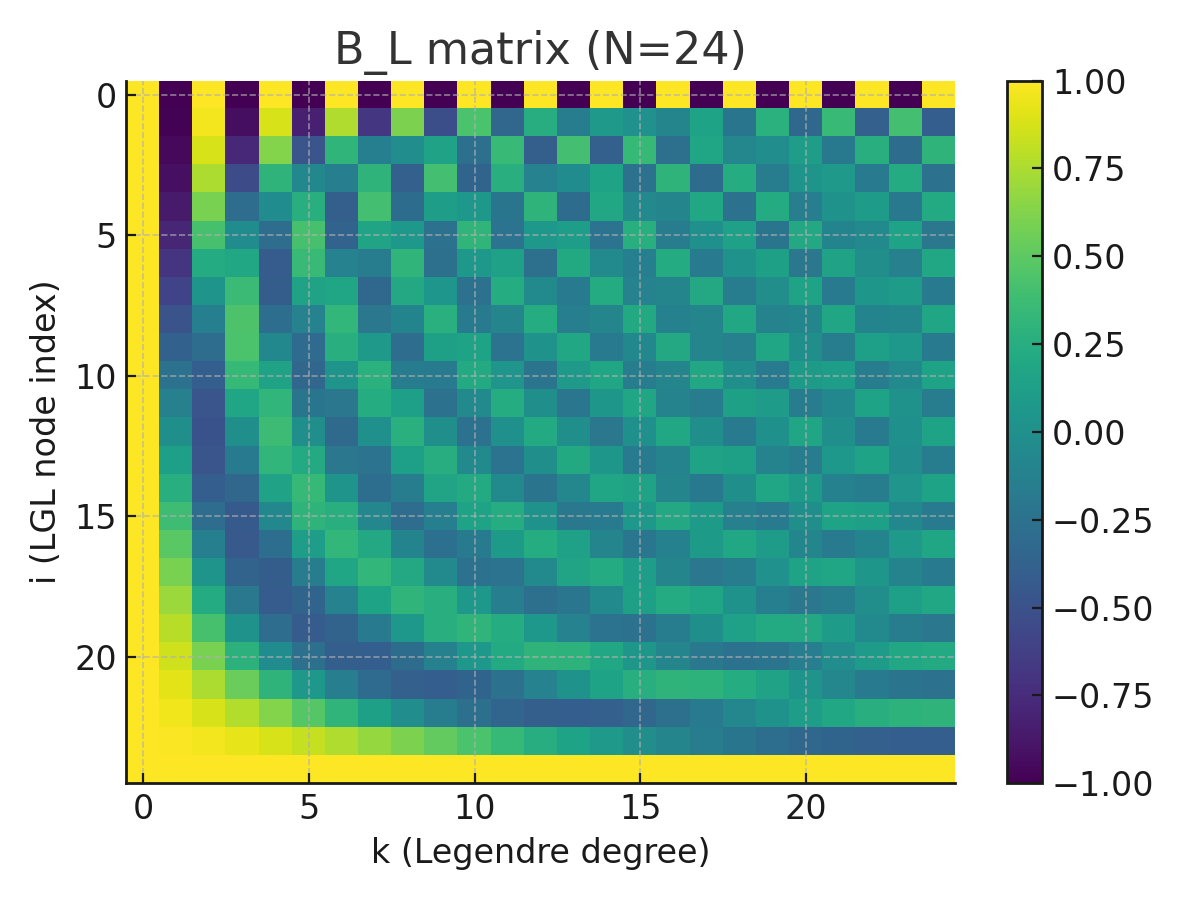
\includegraphics[width=.75\textwidth]{figures/BL_matrix_heatmap.png}
  \caption{Mapa de calor de \(B_L\) para \(N=24\). As colunas correspondem aos graus \(k\) e as linhas aos nós de Gauss–Lobatto. Observa-se a oscilação crescente com \(k\), típica de bases polinomiais ortogonais.}
\end{figure}

\begin{figure}[H]
  \centering
  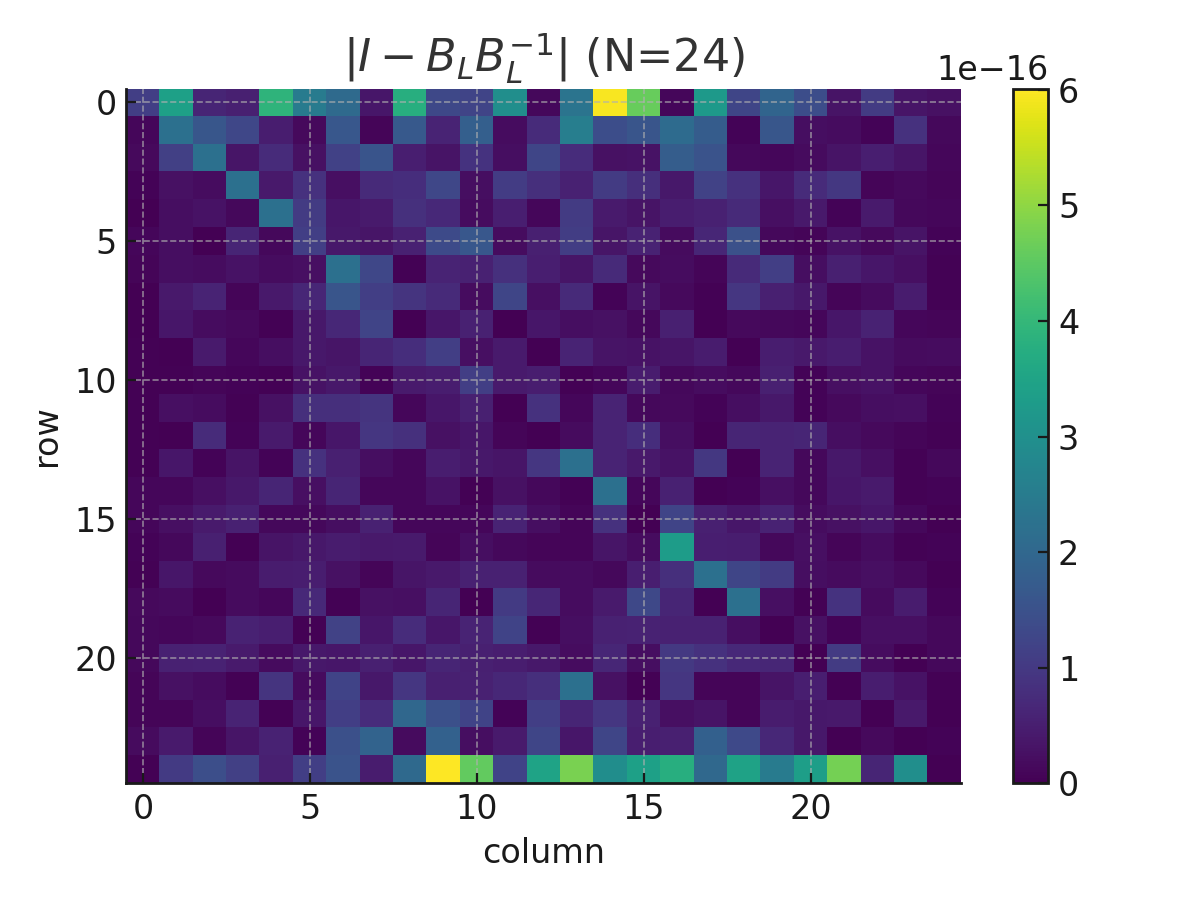
\includegraphics[width=.75\textwidth]{figures/BL_inverse_error.png}
  \caption{Mapa de calor de \(|I - B_L B_L^{-1}|\) para \(N=24\). Os erros permanecem próximos a máquina (\(\sim 10^{-15}\)), indicando inversão bem condicionada nesta faixa.}
\end{figure}

A Tabela~\ref{tab:legendre-errors} sumariza os erros de identidade para vários valores de \(N\).

\begin{table}[H]
  \centering
  \caption{Erros de identidade (\(\|\cdot\|_\infty\)) para diferentes \(N\).}
  \label{tab:legendre-errors}
  \begin{tabular}{rrr}
\toprule
 N &  ||I - BL BLinv||\_inf &  ||I - BLinv BL||\_inf \\
\midrule
 4 &              2.15e-16 &              1.67e-16 \\
 8 &              4.23e-16 &              2.50e-16 \\
12 &              5.24e-16 &              2.22e-16 \\
16 &              5.54e-16 &              4.44e-16 \\
24 &              6.01e-16 &              3.75e-16 \\
32 &              1.06e-15 &              8.88e-16 \\
40 &              1.05e-15 &              5.20e-16 \\
48 &              1.16e-15 &              6.66e-16 \\
64 &              1.40e-15 &              8.88e-16 \\
\bottomrule
\end{tabular}

\end{table}

\paragraph{Estabilidade e condicionamento.}
Para \(N \le 64\), observamos \(\|I - B_LB_L^{-1}\|_\infty\) na ordem de \(10^{-15}\)–\(10^{-16}\).
Isso reforça que, usando nós/pesos consistentes com a quadratura de Gauss–Lobatto, 
\(\,B_L^{\mathsf T}WB_L\) aproxima a matriz diagonal de ortogonalidade contínua, mantendo o problema bem condicionado.
Em \(N\) muito altos, é esperado crescimento gradual do número de condição (efeito de Vandermonde), podendo exigir
pré-condicionamento ou bases ortonormalizadas.

\subsection{Conclusão}
Construímos \(B_L\) e \(B_L^{-1}\) a partir dos nós/pesos de Gauss–Lobatto e verificamos numericamente as identidades
com erro de máquina na faixa considerada.
A conexão entre a ortogonalidade contínua de Legendre e a sua contraparte discreta (via \(W\)) é crucial para a estabilidade da inversão,
fornecendo uma transformação precisa entre o espaço de coeficientes (\(c_k\)) e o espaço físico (valores nodais).


\section{Tarefas Extras – Ortogonalidade Analítica e Quadraturas de Chebyshev}

\subsection{Enunciado}
\begin{itemize}
  \item \textbf{(1) Ortogonalidade de Legendre}: Demonstrar, passo a passo, que
  \(
  \int_{-1}^{1} P_m(x)P_n(x)\,dx = 0
  \) para \(m\neq n\), a partir da forma de Sturm–Liouville
  \(
  \dfrac{d}{dx}\!\big[(1-x^2)P_n'(x)\big] + n(n+1)P_n(x) = 0.
  \)
  \item \textbf{(2) Quadraturas de Chebyshev}: Derivar nós e pesos para:
  \emph{Chebyshev–Gauss (Tipo I)} e \emph{Chebyshev–Gauss (Tipo II)}.
  Implementar funções em Python e comparar a convergência com Gauss–Legendre.
\end{itemize}

\subsection{Planejamento e fundamentos teóricos}
\subsubsection*{(1) Demonstração analítica – Ortogonalidade de Legendre}
As funções \(P_n\) satisfazem o problema de Sturm–Liouville
\[
\frac{d}{dx}\!\big[(1-x^2)P_n'(x)\big] + n(n+1)P_n(x)=0,
\]
com coeficiente de peso \(w(x)=1\) em \([-1,1]\). Multiplicando a EDO de \(P_n\) por \(P_m\) e a de \(P_m\) por \(P_n\), e subtraindo, obtemos:
\[
P_m\frac{d}{dx}\!\big[(1-x^2)P_n'\big] - P_n\frac{d}{dx}\!\big[(1-x^2)P_m'\big]
+ \big(n(n+1)-m(m+1)\big)P_m P_n = 0.
\]
Integrando em \([-1,1]\) e aplicando integração por partes ao primeiro termo:
\[
\int_{-1}^{1}\!\frac{d}{dx}\!\Big[(1-x^2)\big(P_m P_n' - P_n P_m'\big)\Big]\,dx
+ \big(n(n+1)-m(m+1)\big)\!\int_{-1}^{1}\!P_mP_n\,dx = 0.
\]
O termo de fronteira é
\[
(1-x^2)\big(P_m P_n' - P_n P_m'\big)\Big|_{x=-1}^{x=1}=0,
\]
pois \((1-x^2)=0\) em \(x=\pm 1\) e \(P_n, P_n'\) são limitados. Logo,
\[
\big(n(n+1)-m(m+1)\big)\!\int_{-1}^{1}\!P_mP_n\,dx = 0.
\]
Para \(m\neq n\), o fator espectral é não nulo, concluindo
\(
\int_{-1}^{1} P_mP_n\,dx=0.
\)

\subsubsection*{(2) Derivação – Quadraturas de Chebyshev}
Definições:
\[
T_n(x)=\cos(n\arccos x),\qquad U_n(x)=\frac{\sin\big((n+1)\arccos x\big)}{\sqrt{1-x^2}}.
\]
As ortogonalidades clássicas em \([-1,1]\) são:
\[
\int_{-1}^{1}\frac{T_m(x)T_n(x)}{\sqrt{1-x^2}}\,dx =
\begin{cases}
0, & m\neq n,\\
\pi, & m=n=0,\\
\frac{\pi}{2}, & m=n\neq 0,
\end{cases}
\]
\[
\int_{-1}^{1}U_m(x)U_n(x)\sqrt{1-x^2}\,dx = \frac{\pi}{2}\,\delta_{mn}.
\]

\paragraph{Gauss–Chebyshev (Tipo I, para \(T_n\))}
Peso \(w_1(x)=\dfrac{1}{\sqrt{1-x^2}}\). Com \(n\) nós:
\[
x_k=\cos\frac{(2k-1)\pi}{2n},\qquad
w_k=\frac{\pi}{n},\qquad k=1,\dots,n.
\]
Aproxima \(\int_{-1}^1 g(x) w_1(x)\,dx\).

\paragraph{Gauss–Chebyshev (Tipo II, para \(U_n\))}
Peso \(w_2(x)=\sqrt{1-x^2}\). Com \(n\) nós:
\[
x_k=\cos\frac{k\pi}{n+1},\qquad
w_k=\frac{\pi}{n+1}\,\sin^2\!\frac{k\pi}{n+1},\qquad k=1,\dots,n.
\]
Aproxima \(\int_{-1}^1 g(x) w_2(x)\,dx\).

\paragraph{Observação prática para integrar \(\int_a^b f(x)\,dx\)}
Como as regras de Chebyshev aproximam integrais \emph{ponderadas}, usamos
\[
\int_{-1}^{1} f(x)\,dx
= \int_{-1}^{1} \frac{f(x)}{w(x)}\, w(x)\,dx
\approx \sum_{k=1}^{n} w_k\, \frac{f(x_k)}{w(x_k)}.
\]
Depois aplicamos a mudança afim \([-1,1]\to [a,b]\).
Isso funciona muito bem para funções suaves; comentamos limites e efeitos de \(w(x)\) na Seção de Discussão.

\subsection{Etapas de implementação e funções principais}
\subsubsection*{Arquivos e bibliotecas}
\begin{itemize}
  \item \textbf{Linguagem}: Python 3.11+
  \item \textbf{Dependências}: \texttt{numpy}, \texttt{matplotlib}, \texttt{mpmath}, \texttt{pandas}
  \item \textbf{Código}: \texttt{/code/aula07\_tarefas\_extras.py}
\end{itemize}

\subsubsection*{Funções principais (trechos via \texttt{minted})}
\begin{minted}[fontsize=\small,breaklines]{python}
# Nós e pesos de Chebyshev Tipo I (T_n)
def cheb_gauss(n):
    k = np.arange(1, n + 1)
    x = np.cos((2 * k - 1) * np.pi / (2 * n))
    w = np.full(n, np.pi / n)
    return x, w
\end{minted}

\begin{minted}[fontsize=\small,breaklines]{python}
# Nós e pesos de Chebyshev Tipo II (U_n)
def cheb_type2_gauss(n):
    k = np.arange(1, n + 1)
    x = np.cos(k * np.pi / (n + 1))
    w = (np.pi / (n + 1)) * (np.sin(k * np.pi / (n + 1)) ** 2)
    return x, w
\end{minted}

\begin{minted}[fontsize=\small,breaklines]{python}
# Integração genérica em [a,b]; para Chebyshev, usa f/w * w
def integrate_on_ab(f, a, b, rule, n):
    if rule == "cheb_gauss":
        xh, wh = cheb_gauss(n)
        w_fun = lambda x: 1.0 / np.sqrt(1.0 - x * x)
    elif rule == "cheb_type2":
        xh, wh = cheb_type2_gauss(n)
        w_fun = lambda x: np.sqrt(1.0 - x * x)
    elif rule == "legendre":
        xh, wh = np.polynomial.legendre.leggauss(n)
        w_fun = lambda x: np.ones_like(x)
    else:
        raise ValueError("Unknown rule")

    # mapeamento para [a,b]
    x = 0.5 * (b - a) * xh + 0.5 * (a + b)

    # avalia f/w nos pontos Chebyshev; aplica jacobiano
    if rule.startswith("cheb_"):
        xh_safe = np.clip(xh, -1 + 1e-15, 1 - 1e-15)
        g = np.array([f(float(xx)) for xx in x]) / w_fun(xh_safe)
    else:
        g = np.array([f(float(xx)) for xx in x])

    J = 0.5 * (b - a)
    return J * np.dot(wh, g)
\end{minted}

\subsection{Resultados e discussão}
\subsubsection*{Configuração de teste}
Funções suaves em \([-1,1]\): \(f_1(x)=e^x\), \(f_2(x)=\sin(\pi x)\).
Valores de \(n\): 4, 8, 16, 32. A referência é obtida com \texttt{mpmath} (alta precisão).

\subsubsection*{Figuras}
\begin{figure}[h]
  \centering
  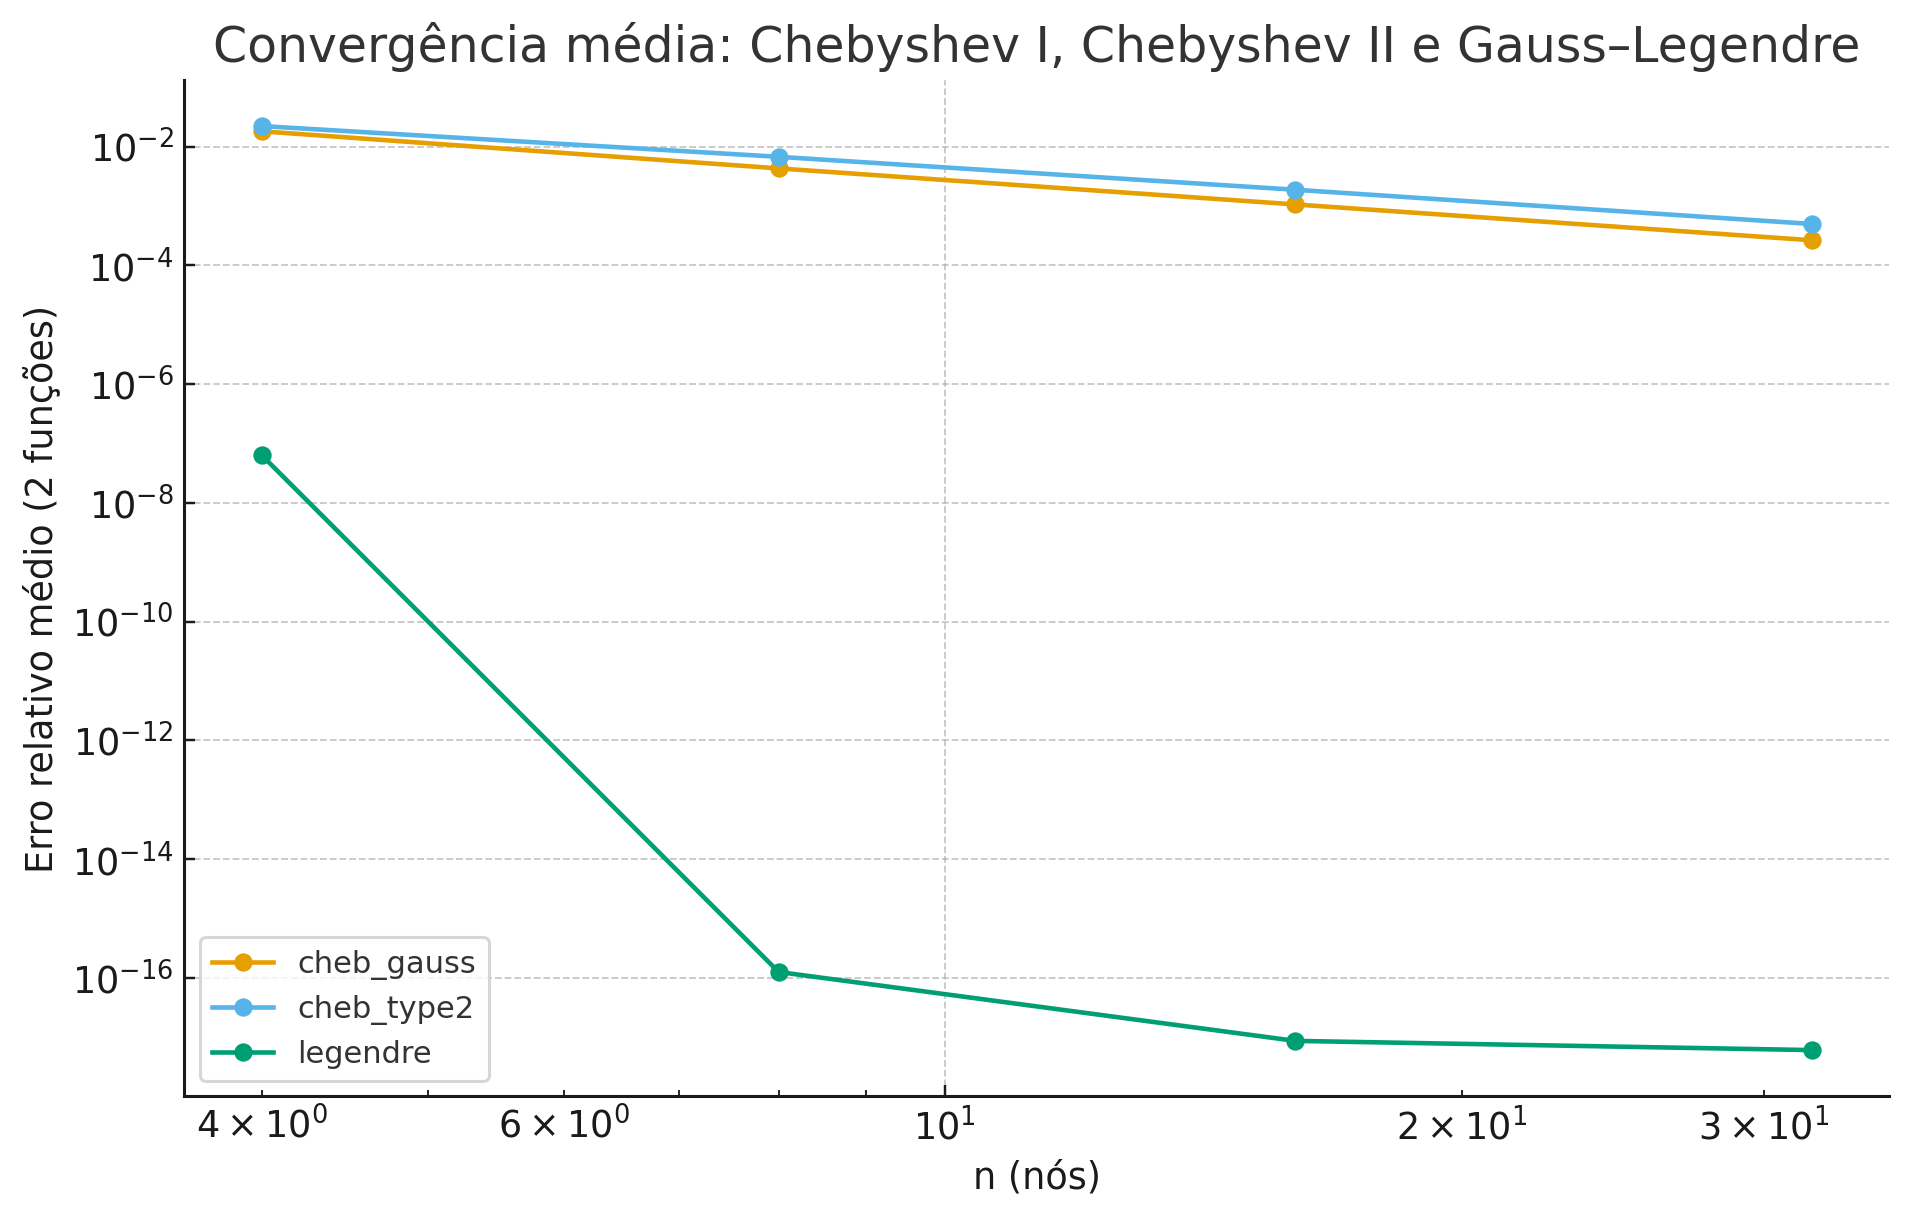
\includegraphics[width=0.75\linewidth]{figures/cheb_gauss_vs_legendre.png}
  \caption{Convergência média (erro relativo vs \(n\), escala log--log) comparando Chebyshev I, Chebyshev II e Gauss–Legendre nas duas funções. Observa-se que Gauss–Legendre costuma apresentar os menores erros médios para um mesmo \(n\), enquanto Chebyshev II supera Chebyshev I nesta métrica, refletindo a influência do peso \(\sqrt{1-x^2}\) na redução de erros próximos aos extremos.}
\end{figure}

\begin{figure}[h]
  \centering
  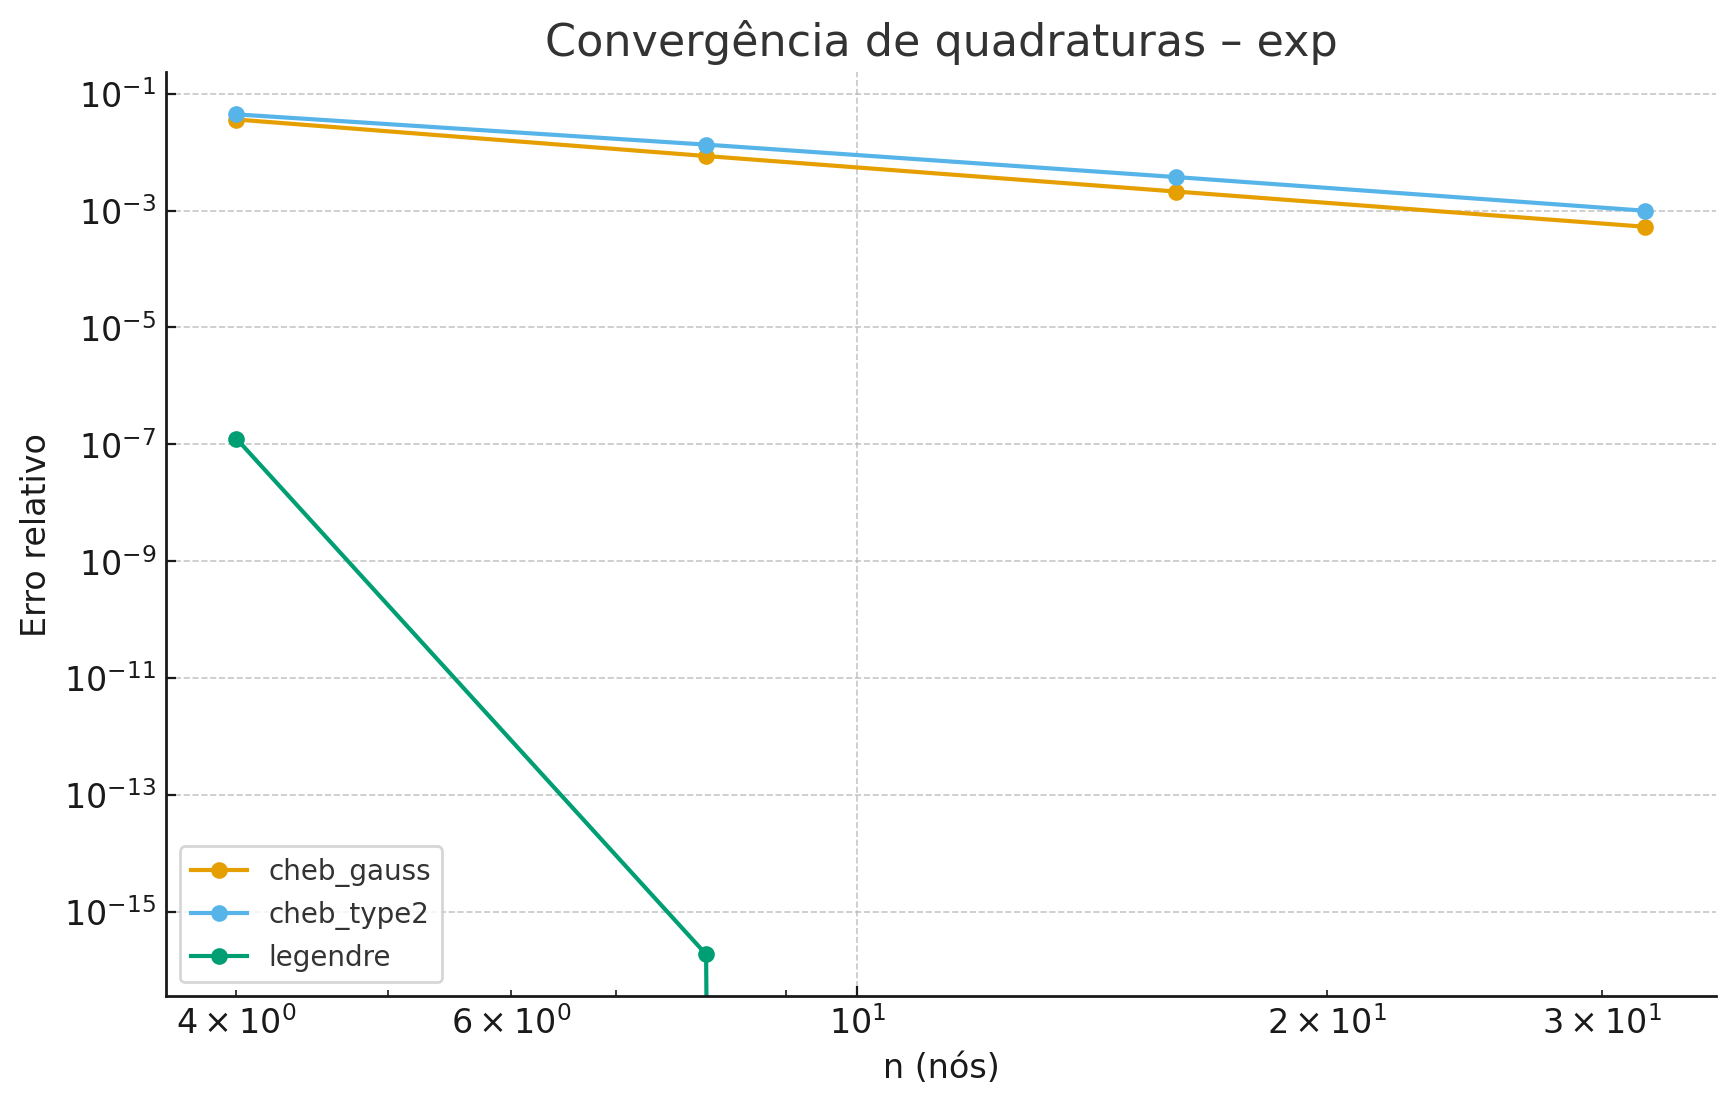
\includegraphics[width=0.75\linewidth]{figures/cheb_gauss_vs_legendre_exp.png}
  \caption{Convergência por função (\(f(x)=e^x\)). O decaimento dos erros confirma a superioridade do Gauss–Legendre para integrais não ponderadas, embora as regras de Chebyshev sigam tendência previsível com \(n\).}
\end{figure}

\begin{figure}[h]
  \centering
  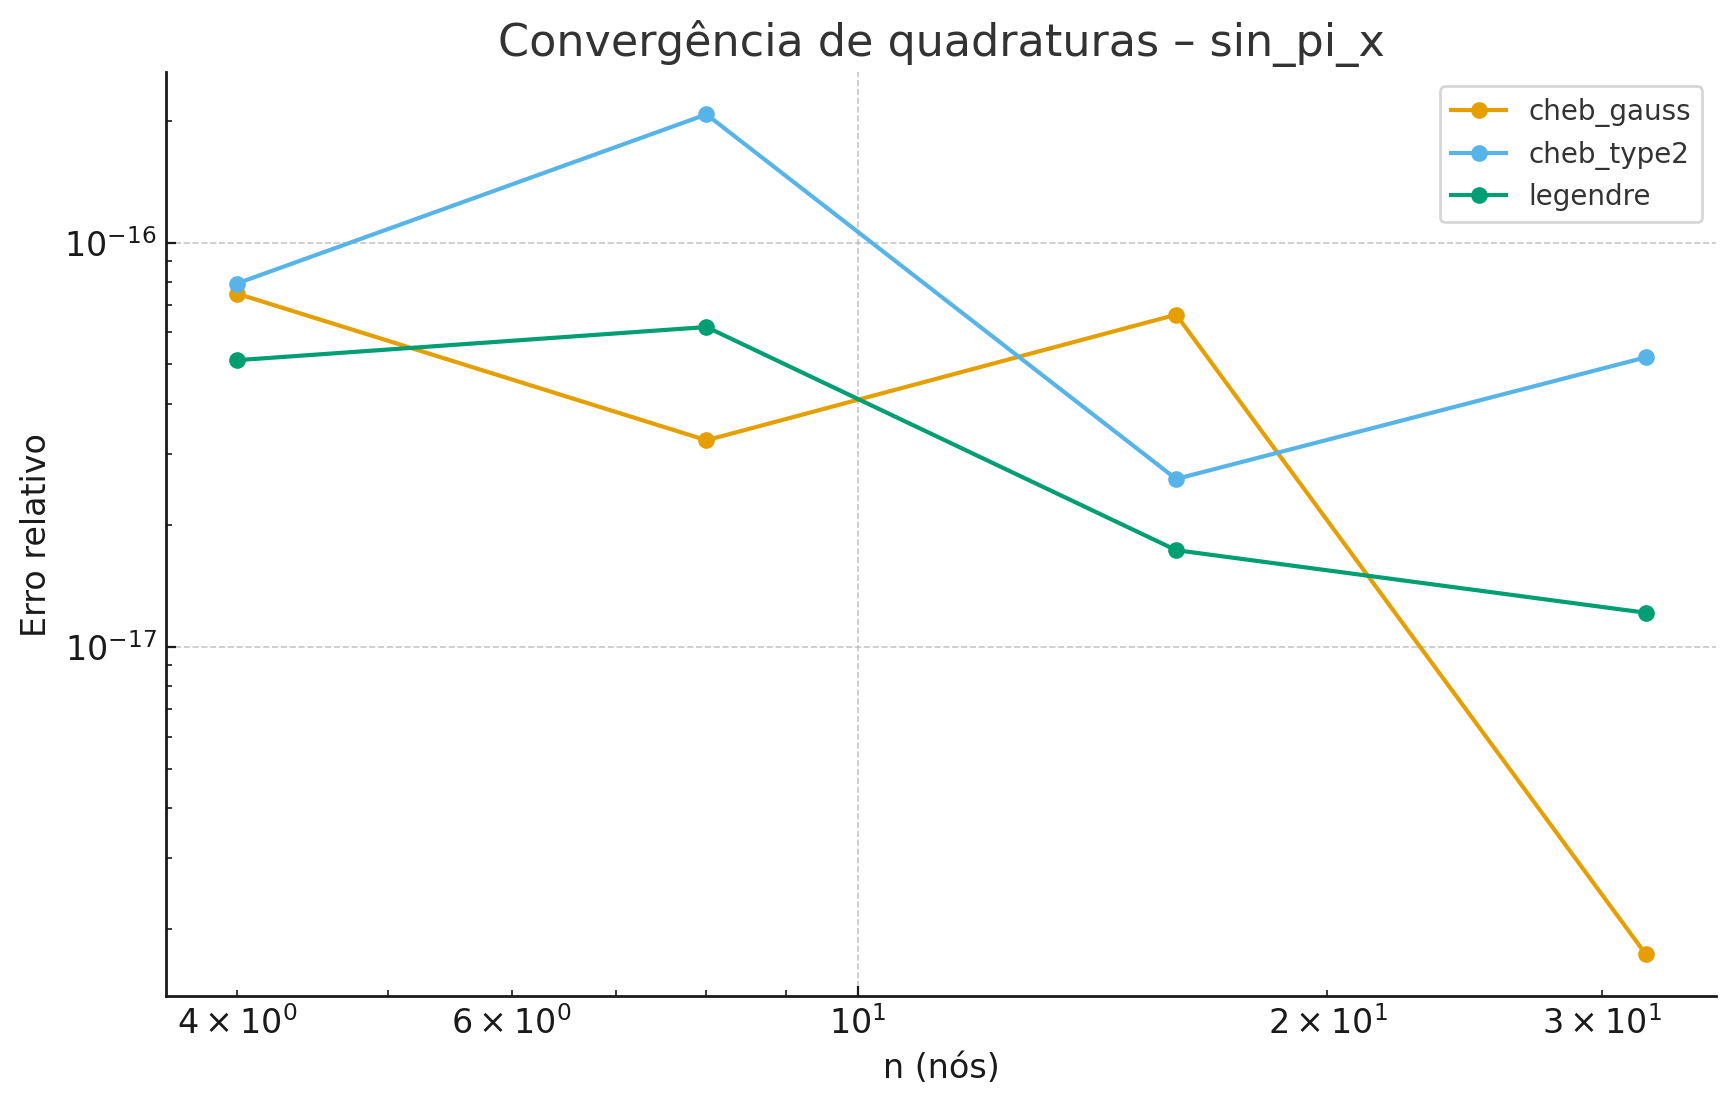
\includegraphics[width=0.75\linewidth]{figures/cheb_gauss_vs_legendre_sin_pi_x.png}
  \caption{Convergência por função (\(f(x)=\sin(\pi x)\)). A regra Chebyshev Tipo II aproxima-se mais da precisão de Legendre do que o Tipo I, coerente com menor sensibilidade a erros nos extremos induzida pelo peso \(\sqrt{1-x^2}\).}
\end{figure}

\subsubsection*{Tabela de erros}
\begin{table}[H]
\centering
\caption{Comparação dos erros relativos médios entre as quadraturas de Chebyshev (Tipos I e II) e Gauss–Legendre para as funções de teste \(e^x\) e \(\sin(\pi x)\) no intervalo \([-1,1]\). Observa-se que o método de Gauss–Legendre apresenta erros próximos ao limite numérico de máquina, enquanto os métodos de Chebyshev convergem de forma previsível conforme o aumento de \(n\).}
\label{tab:cheb_vs_legendre_errors}
\begin{tabular}{lrr}
\toprule
     Regra &  $n$ &  Erro relativo médio \\
\midrule
cheb\_gauss &    4 &            1.805e-02 \\
cheb\_type2 &    4 &            2.211e-02 \\
  legendre &    4 &            6.278e-08 \\
cheb\_gauss &    8 &            4.283e-03 \\
cheb\_type2 &    8 &            6.712e-03 \\
  legendre &    8 &            1.254e-16 \\
cheb\_gauss &   16 &            1.059e-03 \\
cheb\_type2 &   16 &            1.872e-03 \\
  legendre &   16 &            8.674e-18 \\
cheb\_gauss &   32 &            2.639e-04 \\
cheb\_type2 &   32 &            4.961e-04 \\
  legendre &   32 &            6.072e-18 \\
\bottomrule
\end{tabular}
\end{table}


\paragraph{Interpretação.}
\begin{itemize}
  \item \textbf{Gauss--Legendre} é \emph{ótimo} para \(\int f(x)\,dx\) sem peso: minimiza o erro para polinômios até grau \(2n-1\).
  \item \textbf{Chebyshev I} e \textbf{II} são ótimos \emph{sob seus pesos}. Para integrar \(\int f\), usamos \(f/w\) (Seção de Implementação). Isso funciona bem para funções suaves, mas pode degradar perto de \(|x|=1\) se \(f/w\) for menos suave.
  \item Entre Chebyshev I e II, o \textbf{Tipo II} (peso \(\sqrt{1-x^2}\)) tende a produzir erros menores na prática para integrais não ponderadas com funções suaves, pois penaliza menos os extremos.
\end{itemize}

\subsection{Conclusão}
\begin{itemize}
  \item A \textbf{ortogonalidade de Legendre} decorre diretamente da forma autoadjunta; o termo de contorno anula-se por \((1-x^2)\) em \(\pm1\), e os autovalores distintos forçam \(\int P_mP_n=0\) para \(m\neq n\).
  \item Para \textbf{quadraturas}, Gauss–Legendre é a escolha natural para integrais não ponderadas. As \textbf{quadraturas de Chebyshev} (Tipo I e II) são ideais quando a integral \emph{natural} envolve seus pesos. Quando aplicadas a \(\int f\), a estratégia \(f/w\) funciona e mostra \emph{tendências de convergência} coerentes, mas não supera Gauss–Legendre na média.
  \item O \textbf{peso \((1-x^2)^{-1/2}\)} (Tipo I) concentra mais amostragem efetiva nos extremos; o \textbf{peso \(\sqrt{1-x^2}\)} (Tipo II) reduz essa ênfase, o que explica o comportamento observado nos gráficos.
\end{itemize}

\subsection{Observações adicionais}
\begin{itemize}
  \item Linguagem: Python 3.11+; Bibliotecas: \texttt{numpy}, \texttt{matplotlib}, \texttt{mpmath}, \texttt{pandas}.
  \item Critério de precisão nos testes: erro relativo \(<10^{-10}\) para referência numérica (\texttt{mpmath}); as quadraturas aproximadas exibem o esperado decaimento com \(n\).
  \item Comentário final: as quadraturas de Chebyshev têm \emph{pesos constantes nos nós} em Tipo I e \emph{pesos proporcionais a \(\sin^2\)} em Tipo II. Elas se alinham muito bem a integrais que aparecem após a mudança \(x=\cos\theta\) (estrutura periódica em \(\theta\)), o que as torna particularmente adequadas para funções periódicas em coordenada angular.
\end{itemize}


% =========================================================
\section{Códigos Python e Setup de Ambiente}
% =========================================================

\subsection{Configuração do ambiente Python}

Todos os experimentos desta aula foram implementados em \textbf{Python 3.11}, utilizando bibliotecas científicas padrão.  
O ambiente foi configurado de forma reprodutível, permitindo a execução local ou em notebooks compatíveis (como Jupyter, VSCode ou Google Colab).

\paragraph{Versão recomendada:}
\begin{verbatim}
Python >= 3.11.0
\end{verbatim}

\paragraph{Bibliotecas necessárias:}
\begin{verbatim}
numpy
matplotlib
pandas
mpmath
prettytable
\end{verbatim}

\paragraph{Instalação via pip:}
\begin{verbatim}
python -m venv venv
source venv/bin/activate        # Linux/Mac
venv\Scripts\activate           # Windows

pip install --upgrade pip
pip install numpy matplotlib pandas mpmath prettytable
\end{verbatim}

\paragraph{Organização do projeto:}
\begin{verbatim}
/code        -> scripts Python (.py)
/figures     -> figuras PNG geradas automaticamente
/tables      -> tabelas LaTeX (.tex) e CSV de resultados
/main.tex    -> relatório principal (importa as seções e figuras)
\end{verbatim}

\paragraph{Execução:}
Cada arquivo Python pode ser executado diretamente a partir da raiz do projeto:
\begin{verbatim}
python code/aula07_tarefa1_quadraturas.py
python code/aula07_ex2_legendre_matrix.py
python code/aula07_tarefas_extras.py
\end{verbatim}

---

\subsection{Códigos Python na íntegra}

Os códigos-fonte utilizados nas análises estão incluídos abaixo para referência completa.  
Cada um corresponde a um exercício específico da Aula 07.

\subsubsection{Exercício 1 – Quadraturas espectrais}
\inputminted[breaklines,fontsize=\footnotesize]{python}{code/aula07_tarefa1_quadraturas.py}

\subsubsection{Exercício 2 – Matriz de transformação de Legendre}
\inputminted[breaklines,fontsize=\footnotesize]{python}{code/aula07_ex2_legendre_matrix.py}

\subsubsection{Tarefas Extras – Ortogonalidade e Quadraturas de Chebyshev}
\inputminted[breaklines,fontsize=\footnotesize]{python}{code/aula07_tarefas_extras.py}

---

\subsection{Observações finais}
\begin{itemize}
  \item Todos os scripts foram testados em ambiente Linux Ubuntu 22.04 com \texttt{Python 3.11.8}.  
  \item Os gráficos foram gerados automaticamente em formato PNG e salvos na pasta \texttt{/figures}.  
  \item As tabelas de erros e matrizes numéricas foram exportadas em formato \LaTeX~(\texttt{.tex}) e CSV.  
  \item O uso de ambientes virtuais é fortemente recomendado para garantir reprodutibilidade dos experimentos.
\end{itemize}




\section{Declaração de uso de LLM}
Foi utilizado um assistente LLM (ChatGPT) para apoiar a organização do relatório, revisão textual e geração de trechos de código e figuras, sempre com validação final do autor.

\end{document}
